\section[Git work flow]{Git work flow}
\begin{frame}
	\frametitle{Introducing a git work flow}
	\begin{itemize}[<+->]
		\item Working directly on the master branch is not reccommended
		\item In this section I will present a git flow inspired working flow I use at SINTEF:
		\begin{enumerate}[<+->]
			\item Create issue
			\item Create issue branch
			\item Work on issue branch until it works
			\item Create a pull request
			\item Merge issue branch to develop
			\item When develop is stable merge into master
		\end{enumerate}
		\item Example will follow 
	\end{itemize}
\end{frame}
\begin{frame}
	\frametitle{Create an issue}
	\begin{figure}
		\centering
		\begin{overprint}
			\onslide<1>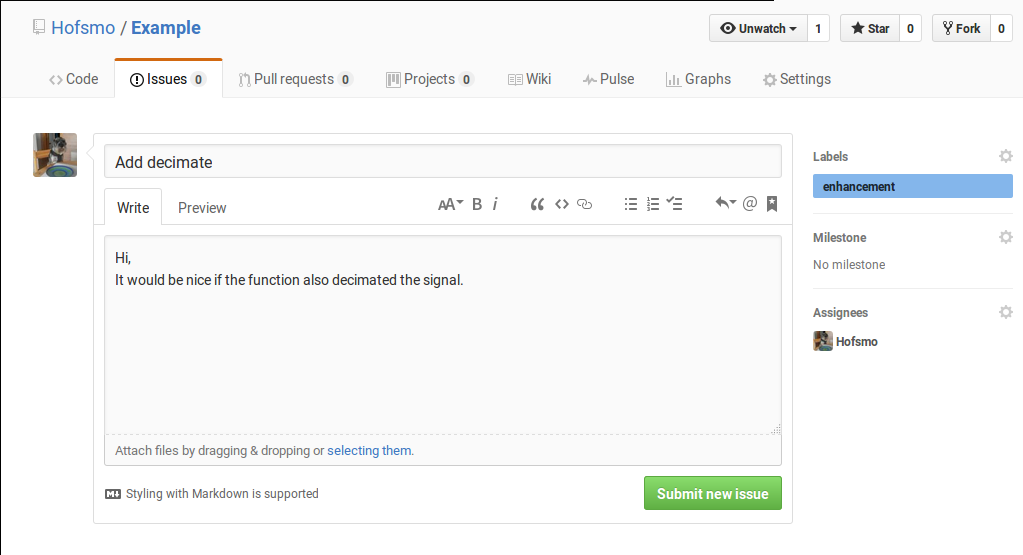
\includegraphics[width=\textwidth]{./pictures/create_issue.png}
			\onslide<2>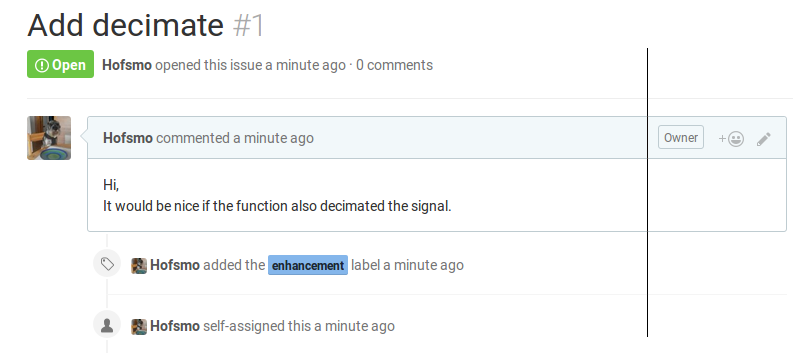
\includegraphics[width=\textwidth]{./pictures/added_issue.png}
		\end{overprint}
	\end{figure}
\end{frame}
\begin{frame}
	\frametitle{Create the feature branches}
	\begin{columns}
		\begin{column}{0.4\textwidth}
			\begin{itemize}[<+->]
				\item Branch the develop branch from master
				\item Develop and master point to the same commit
				\item Branch the feature branch from develop
			\end{itemize}
		\end{column}
		\begin{column}{0.6\textwidth}
			\begin{figure}
				\centering
				\begin{overprint}
					\onslide<1>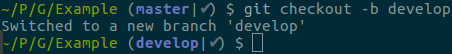
\includegraphics[width=\textwidth]{./pictures/git_branch.png}
					\onslide<2>
\includegraphics[width=\textwidth]{./pictures/develop_branch.png}
					\onslide<3>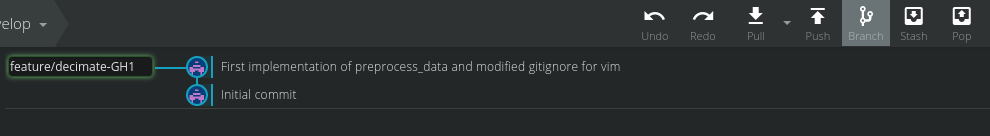
\includegraphics[width=\textwidth]{./pictures/feature_branch.png}
				\end{overprint}
			\end{figure}
		\end{column}
	\end{columns}
\end{frame}
\begin{frame}
	\frametitle{Create a pull request}
	\begin{columns}
		\begin{column}{0.4\textwidth}
			\begin{itemize}[<+->]
				\item Now we can see that we have unstaged changes
				\item Stage the changes
				\item Commit the changes
				\item GH-1 is a reference to the issue
			\end{itemize}
		\end{column}
		\begin{column}{0.6\textwidth}
			\begin{figure}
				\centering
				\begin{overprint}
					\onslide<1>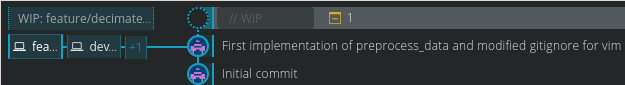
\includegraphics[width=\textwidth]{./pictures/decimate_unstaged.png}
					\onslide<2>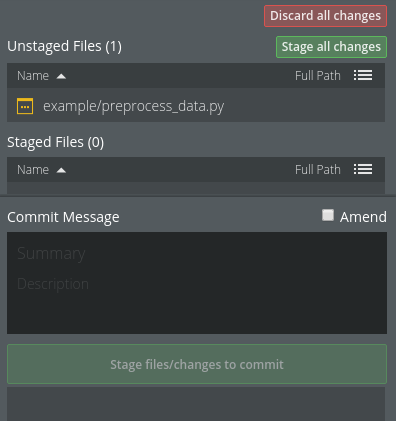
\includegraphics[width=\textwidth]{./pictures/stage_decimate.png}
					\onslide<3>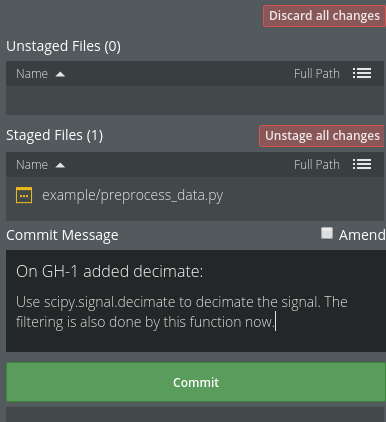
\includegraphics[width=\textwidth]{./pictures/commit_decimate.png}
					\onslide<4>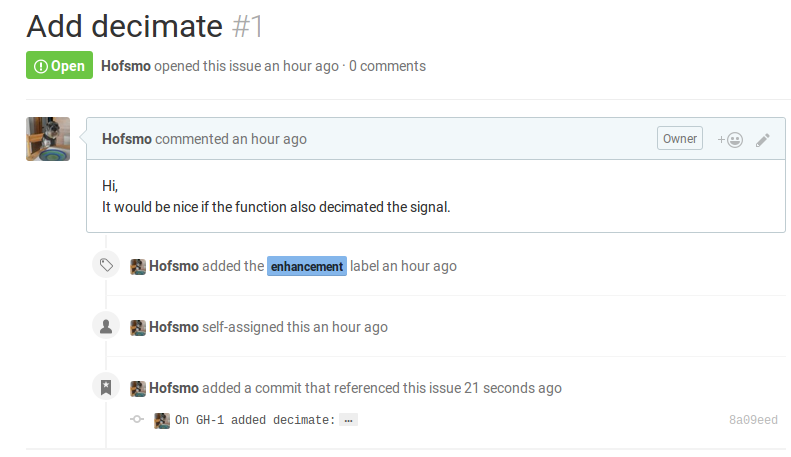
\includegraphics[width=\textwidth]{./pictures/decimate_ref.png}
				\end{overprint}
			\end{figure}
		\end{column}
	\end{columns}
\end{frame}
\begin{frame}
	\frametitle{Create pull request}
	\begin{columns}
		\begin{column}{0.4\textwidth}
			\begin{itemize}[<+->]
				\item Create a pull request
				\item Choose develop as base
				\item Create the pull request
				\item Delete the branch
				\item Close the issue (Could also have written "close GH-1" earlier to do this
				\item The git tree
			\end{itemize}
		\end{column}
		\begin{column}{0.6\textwidth}
			\begin{figure}
				\centering
				\begin{overprint}
					\onslide<1>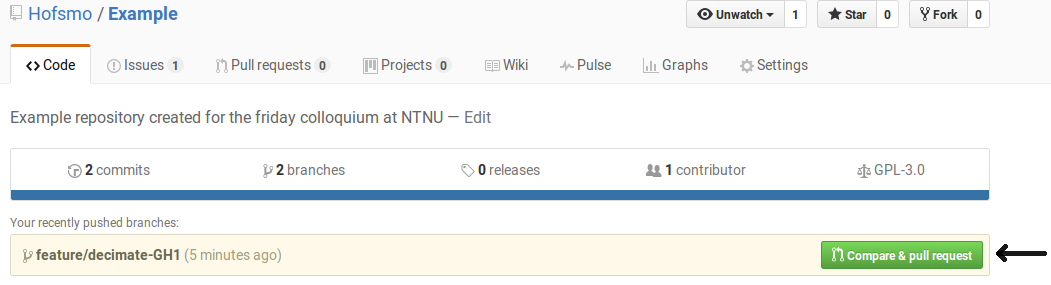
\includegraphics[width=\textwidth]{./pictures/compare_and_pull.png}
					\onslide<2>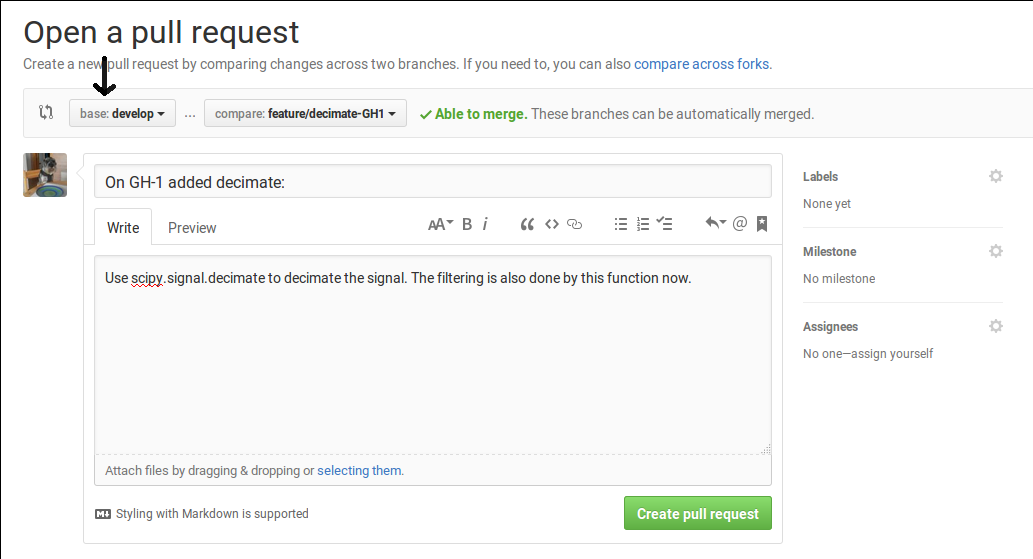
\includegraphics[width=\textwidth]{./pictures/base_develop.png}
					\onslide<3>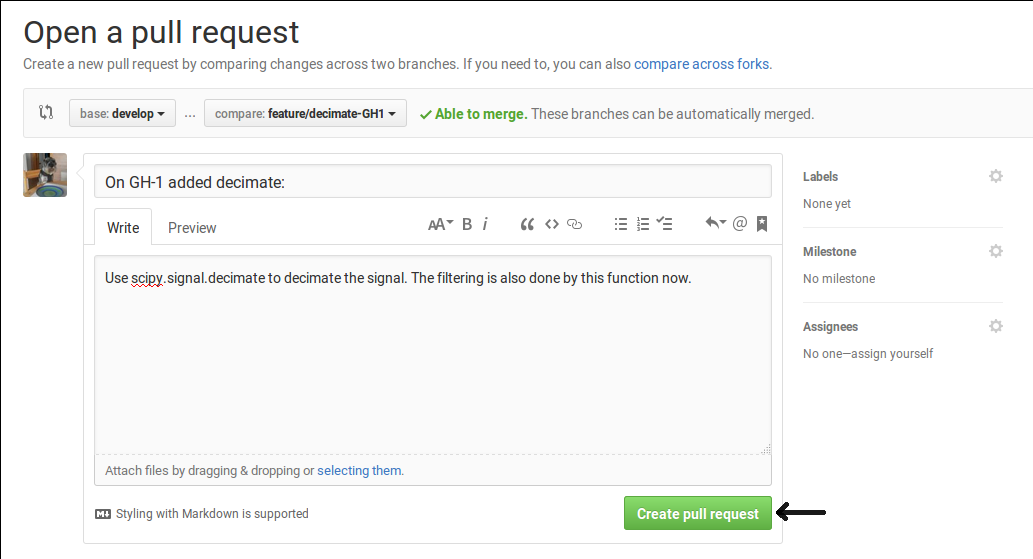
\includegraphics[width=\textwidth]{./pictures/create_pull.png}
					\onslide<4>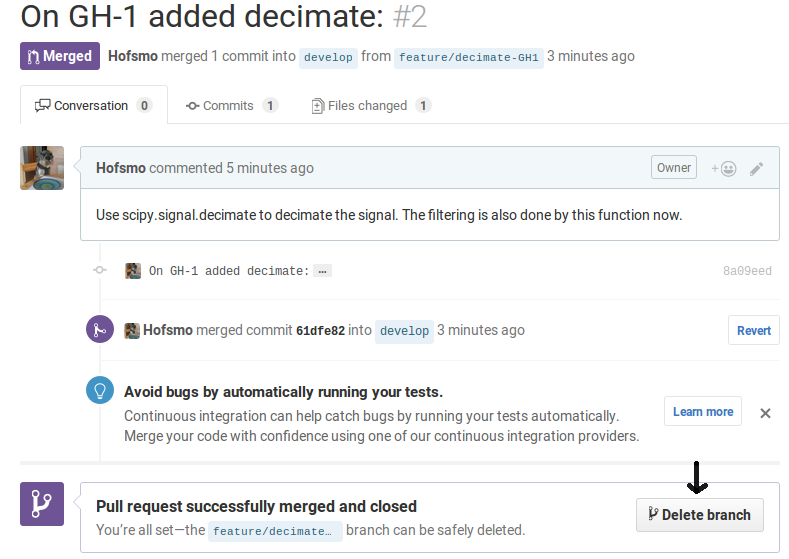
\includegraphics[width=\textwidth]{./pictures/delete_branch.png}
					\onslide<5>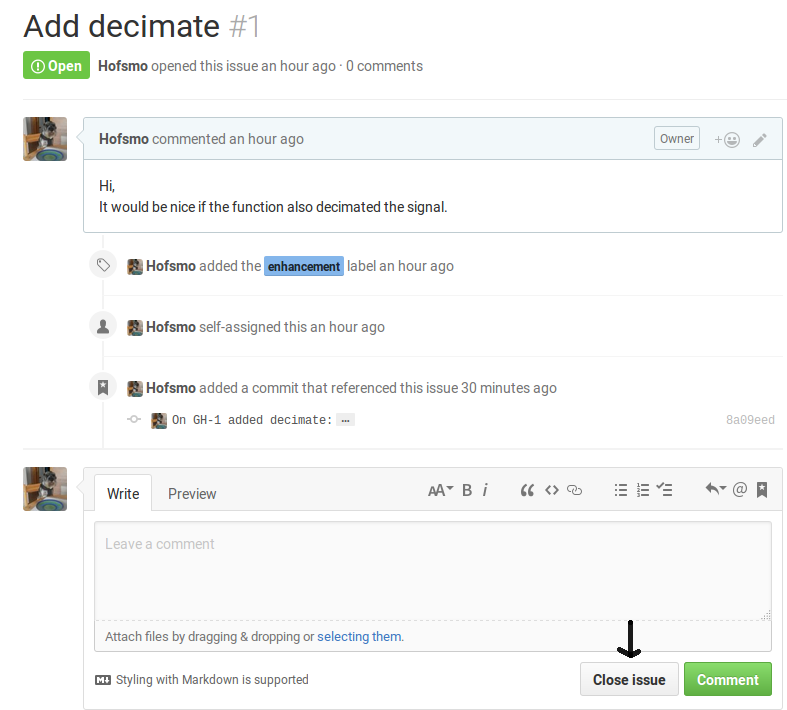
\includegraphics[width=\textwidth]{./pictures/close_issue.png}
					\onslide<6>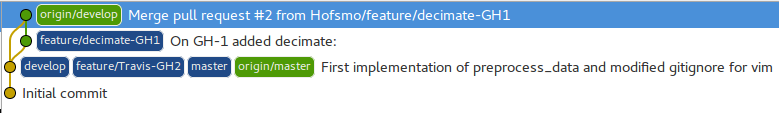
\includegraphics[width=\textwidth]{./pictures/tree.png}
				\end{overprint}
			\end{figure}
		\end{column}
	\end{columns}
\end{frame}
